\documentclass[twocolumn]{article}
\usepackage[utf8]{inputenc}
\usepackage{CJKutf8}
\usepackage{graphicx}

\title{短视频传输实验报告}
\author{计研173 \quad 陈雨兰 \quad 2017310787}
\date{January 2018}

\begin{document}
\begin{CJK*}{UTF8}{gbsn}

\maketitle

\section{算法概述}
\subsection{算法框架}
\begin{figure}[h]
	\centering
	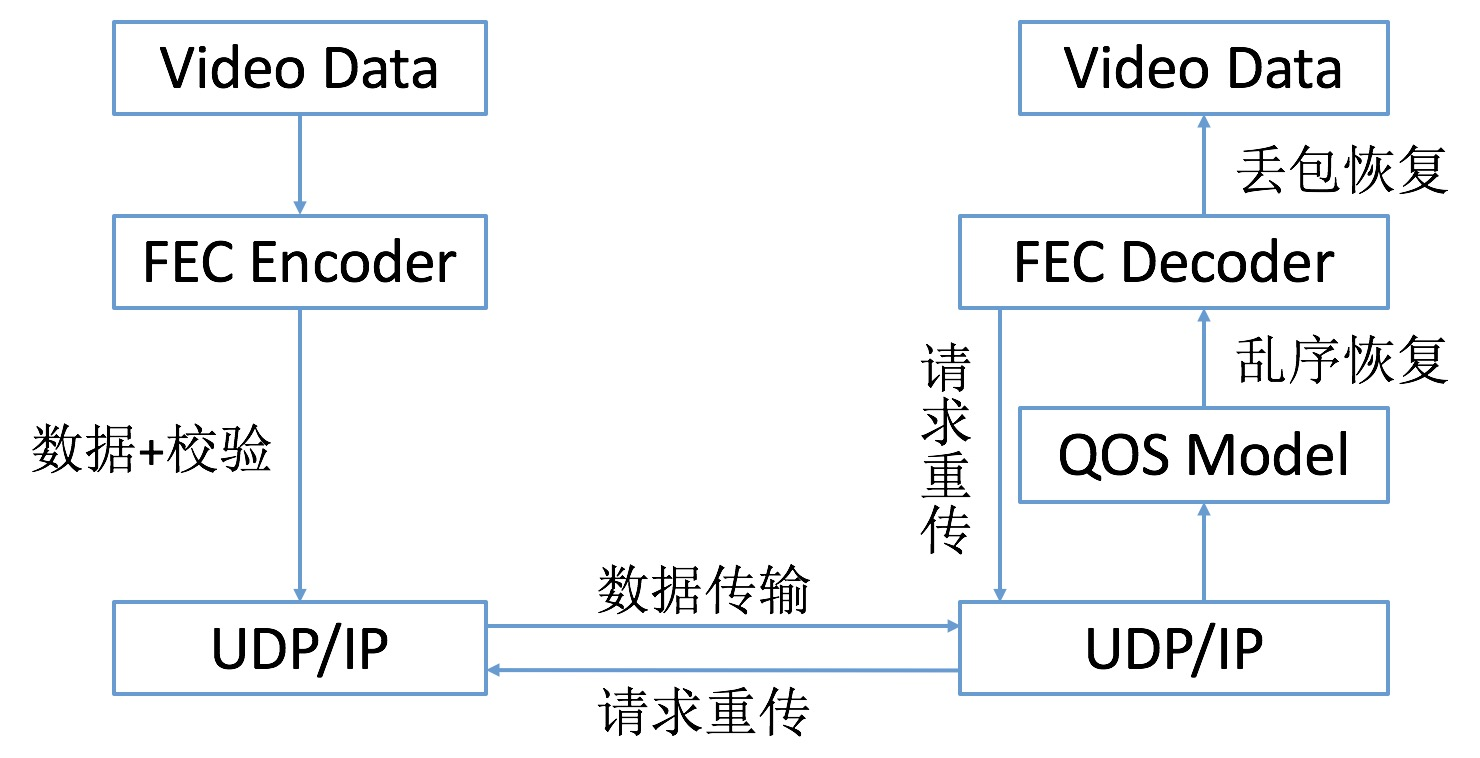
\includegraphics[width=3in]{frame.jpg}
	\caption{算法框架}
	\label{fig:frame}
\end{figure}

\subsection{传输协议}

\subsection{编码协议}
\begin{figure}[h]
	\centering
	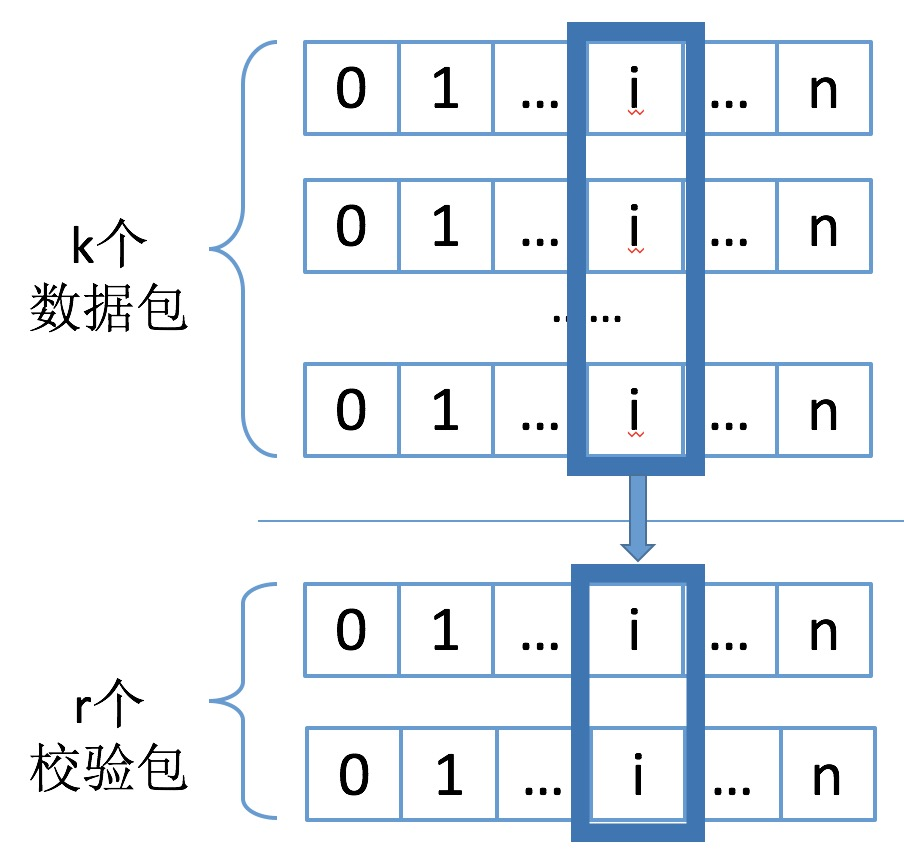
\includegraphics[width=2in]{FEC.jpg}
	\caption{前向纠错算法}
	\label{fig:FEC}
\end{figure}

前向纠错策略(FEC)
每个数据包分为n个字
每个数据包的第i个字为一组,生成校验包
收到任意>=k个包,即可恢复k个数据包
冗余比例:r/k
改进:自适应的冗余比例;
丢失率过高时申请重发


\section{实验结果}
\subsection{传输速度与冗余}
由于使用了前向纠错,算法的冗余度基本相当于前向纠错中校验包的比例。
\subsection{丢包修复能力}
在视频传输中,以固定比例随机丢包,测得算法的丢包比例和修复率之间的关系。

\end{CJK*}
\end{document}
